% Supplementary material. Compile separately; do not append to the 8-page main PDF.
\documentclass[10pt,twocolumn,letterpaper]{article}

\usepackage[pagenumbers]{cvpr}

\definecolor{cvprblue}{rgb}{0.21,0.49,0.74}
\usepackage[pagebackref,breaklinks,colorlinks,allcolors=cvprblue]{hyperref}

\def\paperID{*****}
\def\confName{CVPR}
\def\confYear{2027}

\title{Supplementary Material:\\Detector Ranking is Not Architecture-Invariant\\under Medical Covariate Shift}

\author{Anonymous \confName~submission}

\begin{document}
\maketitle

\section{Leave-one-backbone $W$ is not a CI}

Official Camelyon $W{=}0.694$ ($n{=}8$).
Dropping one backbone and recomputing $W$ on the remaining seven yields $0.676$--$0.738$ (largest increase when dropping ConvNeXt; largest decrease when dropping EffV2-S or RegNet).
This is jackknife \emph{structural} sensitivity of the concordance statistic.
It is not a seed confidence interval and is not written as ``$W{=}0.694$, $95\%$ CI $[\cdot]$.''

\section{HED stain jitter}

Train-only HED stain jitter ($\sigma{=}0.20$, $p{=}1.0$) on ResNet-18, ResNet-50, DenseNet-121, same Adam recipe as official, seed~42.
Precommit dirty-guard: DenseNet hospital-2 MSP ${<}0.80$ ${\Rightarrow}$ dirty.

Hospital-2 MSP: ResNet-18 $0.772$ (enters the $0.695$ band), ResNet-50 $0.593$, DenseNet $0.780$ (\textbf{below $0.80$}).
Gap DenseNet${-}$ResNet-18 ${=}0.008$.
id-val acc ${\ge}0.994$ on all three.
Coverage@risk\,$10\%$ saturates at $1.0$ for these three (not worse than official ResNet-18 $0.145$).
Held-out hospital-1 MSP: ResNet-18 $0.765$, ResNet-50 $0.685$, DenseNet $0.796$.

\textbf{Dirty.}
Part of the apparent gap shrink is DenseNet falling ($0.883{\to}0.780$) while ResNet-18 rises.
Same class as CE{+}SupCon.
Not an open mitigation.
Not expanded to eight CNNs.

\section{MIDOG in-house zoo $n{=}8$ (not official $W$)}

Official MIDOG $W$ remains $n{=}3$, $0.857$.
Five additional in-house CNNs plus the original three, same 1a vs.\ 1b{+}1c protocol, \emph{not} mixed with public OpenMIBOOD R50 ${\sim}0.59$:

\begin{center}
\small
\begin{tabular}{@{}lcc@{}}
\toprule
Backbone & MSP & Maha \\
\midrule
ResNet-18 & 0.438 & 0.733 \\
ResNet-50 & 0.512 & 0.839 \\
DenseNet-121 & 0.447 & 0.910 \\
ConvNeXt-Tiny & 0.521 & 0.801 \\
MobileNetV3-L & 0.469 & 0.714 \\
RegNetY-3.2GF & 0.553 & 0.944 \\
EfficientNet-B3 & 0.486 & 0.673 \\
EfficientNetV2-S@224 & 0.493 & 0.581 \\
\bottomrule
\end{tabular}
\end{center}

MSP $0.44$--$0.55$ on all eight; $0/6$ non-ResNet jumps versus that domain's ResNet mean.
Consistent with official $n{=}3$: no Camelyon-style MSP jump.
A domain-scope bound, not a replacement of official $W$.

\section{Shift-type extract}

Same eight Camelyon seed-42 classifiers; ID ${=}$ Camelyon \texttt{id\_val}.
Arm C ${=}$ hospital-2 (frozen).
Arm T ${=}$ MIDOG 1a (task-shift H\&E).
Arm F ${=}$ CIFAR-10 test (far-OOD).
Extract only; T/F cells are not mixed into official $W$.

\begin{center}
\small
\begin{tabular}{@{}lcl@{}}
\toprule
Arm & non-ResNet jump & readout \\
\midrule
C covariate & $6/6$ & seed-42 count, not multi-seed \\
T task-shift & $\mathbf{0/6}$ & jump disappears \\
F far-OOD & $2/6$ & mixed \\
\bottomrule
\end{tabular}
\end{center}

Joint: \textbf{no law.}
Per-arm Kendall $W$ (8 backbones ${\times}$ 7 methods, never pooled, not official $W$): C $0.731$, T $0.692$, F $0.846$.

\section{Five-seed jumps}

Jump ${=}$ MSP minus that seed's ResNet mean.
Threshold $0.15$.
Official $W$ is seed~42 only.
The MSP matrix is Table~2 of the main paper.

\begin{center}
\small
\setlength{\tabcolsep}{3.5pt}
\begin{tabular}{@{}lccccccc@{}}
\toprule
seed & $R$ mean & Dense & ConvNeXt & Mobile & RegNet & EffB3 & EffV2 \\
\midrule
42 & 0.545 & ${+}0.338$ & ${+}0.301$ & ${+}0.226$ & ${+}0.239$ & ${+}0.258$ & ${+}0.234$ \\
43 & 0.667 & ${+}0.199$ & ${+}0.133$ & ${+}0.061$ & ${+}0.112$ & ${+}0.064$ & ${+}0.077$ \\
44 & 0.610 & ${+}0.258$ & ${+}0.193$ & ${+}0.205$ & ${+}0.226$ & ${+}0.033$ & ${+}0.198$ \\
45 & 0.520 & ${+}0.325$ & ${+}0.244$ & ${+}0.260$ & ${+}0.310$ & ${+}0.298$ & ${+}0.327$ \\
46 & 0.621 & ${+}0.205$ & ${+}0.164$ & ${+}0.124$ & ${+}0.103$ & ${+}0.057$ & ${+}0.214$ \\
\bottomrule
\end{tabular}
\end{center}

\begin{figure*}[t]
\centering
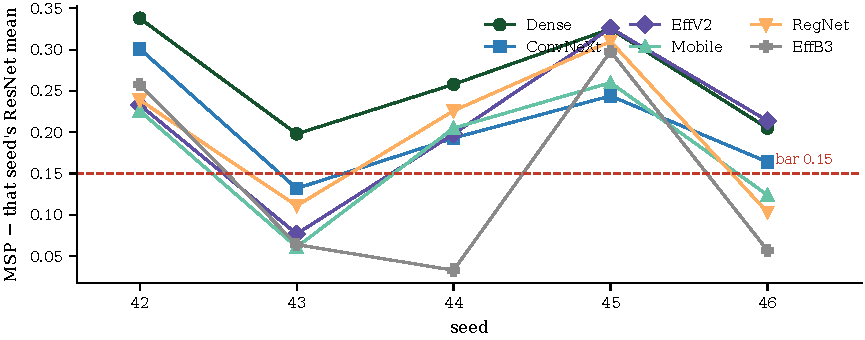
\includegraphics[width=0.92\textwidth]{fig/figA_seed_jumps.pdf}
\caption{Per-seed MSP jump versus that seed's ResNet mean. DenseNet stays above $0.15$ on all five seeds; EfficientNet-B3 does not.}
\end{figure*}

\section{Other closed checks}

ECE, BN-drift, eigenspace summaries, $n_{\mathrm{train}}$ sweeps, and CIFAR-10-C were closed earlier and are not pillars.
CIFAR semantic/far-OOD is not a main-domain result.

\end{document}
